\documentclass[convert]{standalone}

\usepackage{tikz}
\usepackage{graphicx}
\pagestyle{empty}

% INT_AY22_L28-Fig12_Faraday_law_loop.png

\begin{document}
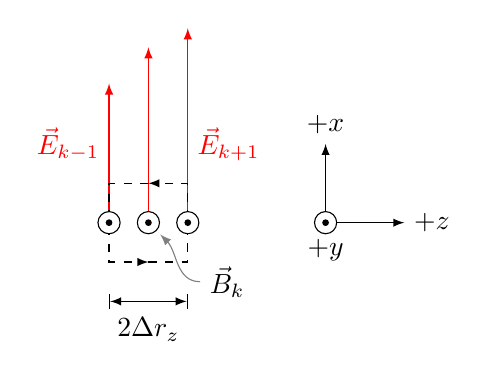
\begin{tikzpicture}[> = latex]

	% Definitions
	
	\def\E{2.5}		% Magnitude of E field
	\def\L{10}		% Wavelength
	
	% Electric field

	\foreach \x in {1.25, 1.75, 2.25}
		\draw [red, ->] (\x, 0) -- (\x, {\E * sin(360 * \x / \L)});
		
	% Labels for E fields
	
	\node [red, left] at (1.25, 1) {${\vec E}_{k - 1}$};
	\node [red, right] at (2.25, 1) {${\vec E}_{k + 1}$}; 
	
	% Loop for Faraday's law
	
	\draw [dashed, ->] (1.75, -0.5) -- (2.25, -0.5) -- (2.25, 0.5) -- (1.75, 0.5);
	\draw [dashed, ->] (1.75, 0.5) -- (1.25, 0.5) -- (1.25, -0.5) -- (1.75, -0.5);
		
	% Magnetic field
	
	\foreach \x in {1.25, 1.75, 2.25}
	{
		\draw [fill = white] (\x, 0) circle (4 pt);
		\filldraw (\x, 0) circle (1 pt);
	}
	
	% Label for B field
	
	\node (B-label) at (2.75, -0.75) {${\vec B}_k$};
	\draw [gray, ->] (B-label.west) to [out = 180, in = 315] (1.9, -0.15);
		
	% Distances between points
	
	\draw [|<->|] (1.25, -1) -- node [below = 0.25 em] {$2 \Delta r_z$} (2.25, -1);
	
	% Coordinate axes
	
	\draw [<->] (4, 1) node [above] {$+x$} -- (4, 0) -- (5, 0) node [right] {$+z$};
	
	\draw [fill = white] (4, 0) circle (4 pt) node [below = 0.25 em] {$+y$};
	\filldraw (4, 0) circle (1 pt);
	
\end{tikzpicture}
\end{document}